\begin{frame}
	\myheading{Module 12.2 : RCNN model for object detection}
\end{frame}

%%%%%%%%%%%%%%%%%%%%%%%%%%%%%%%%%%%%%%%%%%%%%%%%%%%%%%%%%%%%%%%%%%%%%%%%%%%%%%

\begin{frame}
	\begin{center}
		\begin{tikzpicture}[thick,scale=0.6, every node/.style={scale=0.6}]

	\onslide<1->{ % node[below=2]

		\node [text width = 20mm] (F) at (-6.5,7.5) {Input};
		\node[inner sep=0pt] (A) at (-7,6)
		{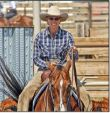
\includegraphics[scale=0.8]{images/cowboy.JPG}};
		\draw[draw=gray,fill=gray,opacity=0.5,thick,solid,rounded corners] (-8.5,4.5) rectangle (-5.5,8);   

	}


	\onslide<1->{ 
		\draw[draw=yellow!50,fill=yellow,thick,solid,rounded corners] (-5,4.5) rectangle (-2,8);  
		\node [text width = 30mm] (F) at (-3.3,7.5) {Region Proposals};
		\node[inner sep=0pt] (B) at (-3.5,6)
		{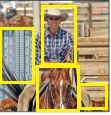
\includegraphics[scale=0.8]{images/c2.jpg}};
		\draw[black, thick, ->] (A) -- (B);     
	}

	\onslide<1->{
		\draw[draw=blue!50,fill=yellow,thick,solid,rounded corners] (-5,4.5) rectangle (-0.8,8);  
		\node [text width = 30mm] (F) at (-2.7,7.5) {Region Proposals};
		\node[inner sep=0pt] (B) at (-3.5,6)
		{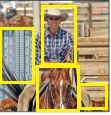
\includegraphics[scale=0.8]{images/c2.jpg}};
		\draw[black, thick, ->] (A) -- (B);     

		\node[inner sep=0pt] (C) at (-1.5,6)
		{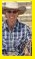
\includegraphics[]{images/c2_crop.jpg}};
		\draw[black,dashed, thick, ->] (-3,6.8) -- (C);     
		\draw[gray,dashed,->] (-3,6) -- (C);      
		\draw[gray,dashed,->] (-3,5) -- (C);     
	}

	\onslide<1->{
		
		\node [text width = 30mm] (F) at (1.5,7.5) {Feature Extraction};
		\node[inner sep=0pt] (D) at (1.4,6)
		{\begin{tikzpicture}[thick,scale=0.6, every node/.style={scale=0.6}]     
			\pgfsetxvec{\pgfpoint{1cm}{0cm}}
			\pgfsetyvec{\pgfpoint{0cm}{1cm}}
			\pgfsetzvec{\pgfpoint{-0.707cm}{.707cm}}     
   
			\onslide<1->{
				\cuboid{(5.9,-2,0.2)}{pink!50}{0.8}{0.8}{0}
				\cuboid{(5.9,-2,0.0)}{pink!50}{0.8}{0.8}{0}
				\cuboid{(5.9,-2,-0.2)}{pink!50}{0.8}{0.8}{0}
				\cuboid{(5.9,-2,-0.4)}{pink!50}{0.8}{0.8}{0}
				\cuboid{(5.9,-2,-0.6)}{pink!50}{0.8}{0.8}{0}
				\cuboid{(5.9,-2,-0.8)}{pink!50}{0.8}{0.8}{0}
				\cuboid{(5.9,-2,-1)}{pink!50}{0.8}{0.8}{0}
				\cuboid{(5.9,-2,-1.2)}{pink!50}{0.8}{0.8}{0}
				\cuboidlabelmine{(5.9,-2,-1.2)}{pink!50}{0.8}{0.8}{0}{10}{10}{}
			}
			\onslide<1->{
         
				\cuboid{(7.9,-2.7,0.8)}{blue!50}{0.5}{0.5}{0}
				\cuboid{(7.9,-2.7,0.6)}{blue!50}{0.5}{0.5}{0}
				\cuboid{(7.9,-2.7,0.4)}{blue!50}{0.5}{0.5}{0}
				\cuboid{(7.9,-2.7,0.2)}{blue!50}{0.5}{0.5}{0}
				\cuboid{(7.9,-2.7,-0.0)}{blue!50}{0.5}{0.5}{0}
				\cuboid{(7.9,-2.7,-0.2)}{blue!50}{0.5}{0.5}{0}
				\cuboid{(7.9,-2.7,-0.4)}{blue!50}{0.5}{0.5}{0}
				\cuboid{(7.9,-2.7,-0.6)}{blue!50}{0.5}{0.5}{0}
				\cuboidlabelmine{(7.9,-2.7,-0.6)}{blue!50}{0.5}{0.5}{0}{5}{5}{}
				\kernel{(6.1,-3,-0.4)}{gray}{0.2}{0.2}{0}{(7.8,-3.2,-0.4)}
			}
			\onslide<1->{
         
				\cuboid{(9.8,-3.5,1.8)}{magenta!50}{0.5}{0}{1.4}
				%   \node at (9.3,-2.85,2.2) {\tiny{FC 1}};
				\draw[black] (7.9,-2.7,0.8) -- (9.55,-3.5,1.78);
				\draw[black] (7.9,-2.7,-0.6) -- (8.8,-3,-0.3);
			}
			\onslide<1->{
				\cuboid{(10.8,-3.5,1.7)}{magenta!50}{0.5}{0}{1.15}
         
				\draw[black] (9.8,-3.5,1.8) -- (10.5,-3.5,1.7);
				\draw[black] (9.8,-3.5,0.4) -- (10.3,-3.5,0.55);
			}
		\end{tikzpicture}};
		\draw[black, thick, ->] (C) -- (D);          
		\draw[draw=gray,fill=gray,opacity=0.5,thick,solid,rounded corners] (-0.4,4.5) rectangle (3.2,8);
	}
	
	\onslide<1->{
	
		\tikzstyle{input_neuron}=[circle,draw=red!50,fill=red!10,thick,minimum size=6mm]
		\tikzstyle{hidden_neuron}=[circle,draw=blue!50,fill=cyan!10,thick,minimum size=6mm]
		\tikzstyle{output_neuron}=[circle,draw=green!50,fill=green!10,thick,minimum size=6mm]
		\tikzstyle{cpy_neuron}=[circle,draw=red!50,fill=red!50,thick,minimum size=6mm]
		\tikzstyle{input}=[circle,draw=black!50,fill=black!20,thick,minimum size=6mm]
	
		
		\node [text width = 30mm] (F) at (5.3,9.5) {Classifier};
		%    \draw (4.5,6.5) rectangle (6.5,8);
		%\node [text width = 25mm] (E) at (4.5,8.2) {Linear Classifier};
		\draw  (3.8,7.85) -- (3.8,9.1);
		\draw  (3.8,7.8) -- (5.2,7.8);
		\node[inner sep=0pt] (I) at (4.5,8.5)
		{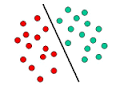
\includegraphics[scale = 0.4,trim={0.5cm 0 0.5cm 0},clip]{images/svm.png}};
	
		\draw[red!100,fill=red!10,thick,solid,rounded corners=10pt] (6,6.7) rectangle (7,9.8);
	
		\node [hidden_neuron] (neuron51) at (6.5,9.2) {} ;
		\node [hidden_neuron] (neuron52) at (6.5,8.5)  {};
		\node at (6.5,7.9) {\vdots};
		\node [hidden_neuron] (neuron53) at (6.5,7.2)  {};
		\node [cpy_neuron] (neuron01) at (6.5,8.5) {};
	
		\draw [->] (I) -- (neuron01);
		\draw  (2.7,6) -- (2.7,7);
		\draw  (2.7,7) -- (4.2,7);
		\draw [->]  (4.2,7) -- (4.2,7.8);
		\draw[draw=gray,fill=gray,opacity=0.5,thick,solid,rounded corners] (3.6,10) rectangle (7.2,6.5);
	}
	
	
	\onslide<1->{
	
		
		\node [text width = 30mm] (F) at (5.3,5.6) {Bounding Box Regression};
	
		\node[inner sep=0pt] (A) at (5.2,4.2)
		{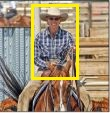
\includegraphics[scale = 0.6]{images/cowboy_cr.jpg}};
	
		\draw  (1.6,5.5) -- (1.6,4);
		\draw [->] (1.6,4) -- (4.2,4);
		\draw[draw=gray,fill=gray,opacity=0.5,thick,solid,rounded corners] (3.6,3.1) rectangle (7.2,6.2);
	}

\end{tikzpicture}
	\end{center}
	
	\begin{columns}
		\column{0.4\textwidth}
		\vspace{-1cm}
		\begin{overlayarea}{\textwidth}{\textheight}
			\only<2>{
				\begin{figure}[H]
					\centering
					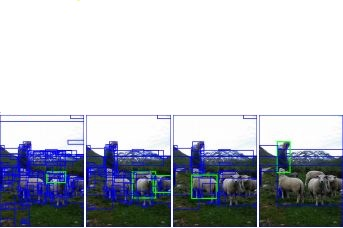
\includegraphics[scale= 0.6]{images/CNN2_1_first.JPG}
				\end{figure}}
		    \only<3->{
   				\begin{figure}[H]
   					\centering
   					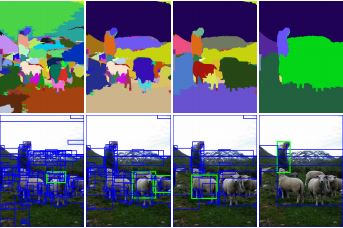
\includegraphics[scale= 0.6]{images/CNN2_1.JPG}
   				\end{figure}}
		\end{overlayarea}
		
		\column{0.6\textwidth}
		\begin{overlayarea}{\textwidth}{\textheight}
			
			\begin{itemize}
				\justifying
				\item<2-> \textbf{Selective Search} for region proposals 
				\item<3-> Does hierarchical clustering at different scales 
				\item<4-> For example the figures from left to right show clusters of increasing sizes
				\item<5-> Such a hierarchical clustering is important as we may find different objects at different scales 
			\end{itemize}
		\end{overlayarea}
	\end{columns}
\end{frame}

%%%%%%%%%%%%%%%%%%%%%%%%%%%%%%%%%%%%%%%%%%%%%%%%%%%%%%%%%%%%%%%%%%%%%%%%%%%%%%

\begin{frame}
	\begin{center}
		\begin{tikzpicture}[thick,scale=0.6, every node/.style={scale=0.6}]

	\onslide<1->{ % node[below=2]

		\node [text width = 20mm] (F) at (-6.5,7.5) {Input};
		\node[inner sep=0pt] (A) at (-7,6)
		{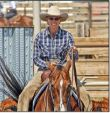
\includegraphics[scale=0.8]{images/cowboy.JPG}};
		\draw[draw=gray,fill=gray,opacity=0.5,thick,solid,rounded corners] (-8.5,4.5) rectangle (-5.5,8);   

	}


	\onslide<1->{ 
		\draw[draw=yellow!50,fill=yellow,thick,solid,rounded corners] (-5,4.5) rectangle (-2,8);  
		\node [text width = 30mm] (F) at (-3.3,7.5) {Region Proposals};
		\node[inner sep=0pt] (B) at (-3.5,6)
		{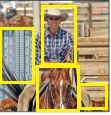
\includegraphics[scale=0.8]{images/c2.jpg}};
		\draw[black, thick, ->] (A) -- (B);     
	}

	\onslide<1->{
		\draw[draw=blue!50,fill=yellow,thick,solid,rounded corners] (-5,4.5) rectangle (-0.8,8);  
		\node [text width = 30mm] (F) at (-2.7,7.5) {Region Proposals};
		\node[inner sep=0pt] (B) at (-3.5,6)
		{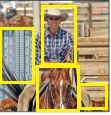
\includegraphics[scale=0.8]{images/c2.jpg}};
		\draw[black, thick, ->] (A) -- (B);     

		\node[inner sep=0pt] (C) at (-1.5,6)
		{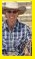
\includegraphics[]{images/c2_crop.jpg}};
		\draw[black,dashed, thick, ->] (-3,6.8) -- (C);     
		\draw[gray,dashed,->] (-3,6) -- (C);      
		\draw[gray,dashed,->] (-3,5) -- (C);     
	}

	\onslide<1->{
		
		\node [text width = 30mm] (F) at (1.5,7.5) {Feature Extraction};
		\node[inner sep=0pt] (D) at (1.4,6)
		{\begin{tikzpicture}[thick,scale=0.6, every node/.style={scale=0.6}]     
			\pgfsetxvec{\pgfpoint{1cm}{0cm}}
			\pgfsetyvec{\pgfpoint{0cm}{1cm}}
			\pgfsetzvec{\pgfpoint{-0.707cm}{.707cm}}     
   
			\onslide<1->{
				\cuboid{(5.9,-2,0.2)}{pink!50}{0.8}{0.8}{0}
				\cuboid{(5.9,-2,0.0)}{pink!50}{0.8}{0.8}{0}
				\cuboid{(5.9,-2,-0.2)}{pink!50}{0.8}{0.8}{0}
				\cuboid{(5.9,-2,-0.4)}{pink!50}{0.8}{0.8}{0}
				\cuboid{(5.9,-2,-0.6)}{pink!50}{0.8}{0.8}{0}
				\cuboid{(5.9,-2,-0.8)}{pink!50}{0.8}{0.8}{0}
				\cuboid{(5.9,-2,-1)}{pink!50}{0.8}{0.8}{0}
				\cuboid{(5.9,-2,-1.2)}{pink!50}{0.8}{0.8}{0}
				\cuboidlabelmine{(5.9,-2,-1.2)}{pink!50}{0.8}{0.8}{0}{10}{10}{}
			}
			\onslide<1->{
         
				\cuboid{(7.9,-2.7,0.8)}{blue!50}{0.5}{0.5}{0}
				\cuboid{(7.9,-2.7,0.6)}{blue!50}{0.5}{0.5}{0}
				\cuboid{(7.9,-2.7,0.4)}{blue!50}{0.5}{0.5}{0}
				\cuboid{(7.9,-2.7,0.2)}{blue!50}{0.5}{0.5}{0}
				\cuboid{(7.9,-2.7,-0.0)}{blue!50}{0.5}{0.5}{0}
				\cuboid{(7.9,-2.7,-0.2)}{blue!50}{0.5}{0.5}{0}
				\cuboid{(7.9,-2.7,-0.4)}{blue!50}{0.5}{0.5}{0}
				\cuboid{(7.9,-2.7,-0.6)}{blue!50}{0.5}{0.5}{0}
				\cuboidlabelmine{(7.9,-2.7,-0.6)}{blue!50}{0.5}{0.5}{0}{5}{5}{}
				\kernel{(6.1,-3,-0.4)}{gray}{0.2}{0.2}{0}{(7.8,-3.2,-0.4)}
			}
			\onslide<1->{
         
				\cuboid{(9.8,-3.5,1.8)}{magenta!50}{0.5}{0}{1.4}
				%   \node at (9.3,-2.85,2.2) {\tiny{FC 1}};
				\draw[black] (7.9,-2.7,0.8) -- (9.55,-3.5,1.78);
				\draw[black] (7.9,-2.7,-0.6) -- (8.8,-3,-0.3);
			}
			\onslide<1->{
				\cuboid{(10.8,-3.5,1.7)}{magenta!50}{0.5}{0}{1.15}
         
				\draw[black] (9.8,-3.5,1.8) -- (10.5,-3.5,1.7);
				\draw[black] (9.8,-3.5,0.4) -- (10.3,-3.5,0.55);
			}
		\end{tikzpicture}};
		\draw[black, thick, ->] (C) -- (D);          
		\draw[draw=gray,fill=gray,opacity=0.5,thick,solid,rounded corners] (-0.4,4.5) rectangle (3.2,8);
	}
	
	\onslide<1->{
	
		\tikzstyle{input_neuron}=[circle,draw=red!50,fill=red!10,thick,minimum size=6mm]
		\tikzstyle{hidden_neuron}=[circle,draw=blue!50,fill=cyan!10,thick,minimum size=6mm]
		\tikzstyle{output_neuron}=[circle,draw=green!50,fill=green!10,thick,minimum size=6mm]
		\tikzstyle{cpy_neuron}=[circle,draw=red!50,fill=red!50,thick,minimum size=6mm]
		\tikzstyle{input}=[circle,draw=black!50,fill=black!20,thick,minimum size=6mm]
	
		
		\node [text width = 30mm] (F) at (5.3,9.5) {Classifier};
		%    \draw (4.5,6.5) rectangle (6.5,8);
		%\node [text width = 25mm] (E) at (4.5,8.2) {Linear Classifier};
		\draw  (3.8,7.85) -- (3.8,9.1);
		\draw  (3.8,7.8) -- (5.2,7.8);
		\node[inner sep=0pt] (I) at (4.5,8.5)
		{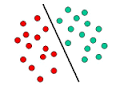
\includegraphics[scale = 0.4,trim={0.5cm 0 0.5cm 0},clip]{images/svm.png}};
	
		\draw[red!100,fill=red!10,thick,solid,rounded corners=10pt] (6,6.7) rectangle (7,9.8);
	
		\node [hidden_neuron] (neuron51) at (6.5,9.2) {} ;
		\node [hidden_neuron] (neuron52) at (6.5,8.5)  {};
		\node at (6.5,7.9) {\vdots};
		\node [hidden_neuron] (neuron53) at (6.5,7.2)  {};
		\node [cpy_neuron] (neuron01) at (6.5,8.5) {};
	
		\draw [->] (I) -- (neuron01);
		\draw  (2.7,6) -- (2.7,7);
		\draw  (2.7,7) -- (4.2,7);
		\draw [->]  (4.2,7) -- (4.2,7.8);
		\draw[draw=gray,fill=gray,opacity=0.5,thick,solid,rounded corners] (3.6,10) rectangle (7.2,6.5);
	}


	\onslide<1->{
	
		
		\node [text width = 30mm] (F) at (5.3,5.6) {Bounding Box Regression};
	
		\node[inner sep=0pt] (A) at (5.2,4.2)
		{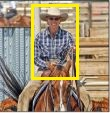
\includegraphics[scale = 0.6]{images/cowboy_cr.jpg}};
	
		\draw  (1.6,5.5) -- (1.6,4);
		\draw [->] (1.6,4) -- (4.2,4);
		\draw[draw=gray,fill=gray,opacity=0.5,thick,solid,rounded corners] (3.6,3.1) rectangle (7.2,6.2);
	}

\end{tikzpicture}

	\end{center}

	\vspace{-0.5cm}
	\begin{columns}
		\column{0.4\textwidth}
		\begin{overlayarea}{\textwidth}{\textheight}
			\begin{center}
				\begin{tikzpicture}[scale=0.8, transform shape]
	\onslide<1->{ % node[below=2]
		
		\draw[draw=blue!50,fill=cyan!10,thick,solid,rounded corners] (3.3,4.6) rectangle (0.7,7.3);    

		\node[inner sep=0pt] (A) at (2,6)
		{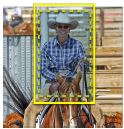
\includegraphics[scale=0.7]{images/CNN_cowboy.JPG}};}

	\onslide<2->{
		\draw[draw=blue!50,fill=cyan!10,thick,solid,rounded corners] (5.3,4.8) rectangle (3.7,7.2);    

		\node[inner sep=0pt] (B) at (4.5,6)
		{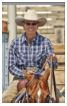
\includegraphics[scale=0.7]{images/CNN_cowboy_crop.JPG}};
		\node at (4.5,4.5) {};}
	\onslide<2->{\draw[black, thick, ->]  (3.2,6) --  (3.9,6);} 
	
	
	\onslide<3->{
		\draw[draw=blue!50,fill=cyan!10,thick,solid,rounded corners] (8.3,4.8) rectangle (5.9,7.2);    

		\node[inner sep=0pt] (C) at (7.1,6)
		{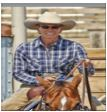
\includegraphics[scale=0.7]{images/CNN_cowboy_scale.JPG}};
		\node [text width=35mm] at (7.8,4) {};
	}
	\onslide<3->{\draw[black, thick, ->]  (5.2,6) --  (6.1,6);} 
	
\end{tikzpicture}

			\end{center}
			
		\end{overlayarea}
		
		\column{0.6\textwidth}
		\begin{overlayarea}{\textwidth}{\textheight}
			\vspace{0.5cm}
			\begin{itemize}
				\justifying
				\item<2-> Proposed regions are cropped to form mini images
				\item<3-> Each mini image is scaled to match the CNN's (feature extractor) input size 
			\end{itemize}  
		\end{overlayarea}     
	\end{columns}
\end{frame}

%%%%%%%%%%%%%%%%%%%%%%%%%%%%%%%%%%%%%%%%%%%%%%%%%%%%%%%%%%%%%%%%%%%%%%%%%%%%%%

\begin{frame}
	\begin{center}
		\begin{tikzpicture}[thick,scale=0.6, every node/.style={scale=0.6}]

	\onslide<1->{ % node[below=2]

		\node [text width = 20mm] (F) at (-6.5,7.5) {Input};
		\node[inner sep=0pt] (A) at (-7,6)
		{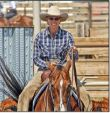
\includegraphics[scale=0.8]{images/cowboy.JPG}};
		\draw[draw=gray,fill=gray,opacity=0.5,thick,solid,rounded corners] (-8.5,4.5) rectangle (-5.5,8);   
       
	}

	\onslide<1->{

		\node [text width = 30mm] (F) at (-2.7,7.5) {Region Proposals};
		\node[inner sep=0pt] (B) at (-3.5,6)
		{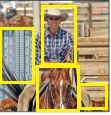
\includegraphics[scale=0.8]{images/c2.jpg}};
		\draw[black, thick, ->] (A) -- (B);     

		\node[inner sep=0pt] (C) at (-1.5,6)
		{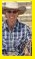
\includegraphics[]{images/c2_crop.jpg}};
		\draw[black,dashed, thick, ->] (-3,6.8) -- (C);     
		\draw[gray,dashed,->] (-3,6) -- (C);      
		\draw[gray,dashed,->] (-3,5) -- (C);     
		\draw[draw=gray,fill=gray,opacity=0.5,thick,solid,rounded corners] (-5,4.5) rectangle (-0.8,8);     
	}

	\onslide<1->{
		\draw[draw=blue!50,fill=yellow,thick,solid,rounded corners] (-0.4,4.5) rectangle (3.2,8);
		\node [text width = 30mm] (F) at (1.5,7.5) {Feature Extraction};
		\node[inner sep=0pt] (D) at (1.4,6)
		{\begin{tikzpicture}[thick,scale=0.6, every node/.style={scale=0.6}]     
			\pgfsetxvec{\pgfpoint{1cm}{0cm}}
			\pgfsetyvec{\pgfpoint{0cm}{1cm}}
			\pgfsetzvec{\pgfpoint{-0.707cm}{.707cm}}     
   
			\onslide<1->{
				\cuboid{(5.9,-2,0.2)}{pink!50}{0.8}{0.8}{0}
				\cuboid{(5.9,-2,0.0)}{pink!50}{0.8}{0.8}{0}
				\cuboid{(5.9,-2,-0.2)}{pink!50}{0.8}{0.8}{0}
				\cuboid{(5.9,-2,-0.4)}{pink!50}{0.8}{0.8}{0}
				\cuboid{(5.9,-2,-0.6)}{pink!50}{0.8}{0.8}{0}
				\cuboid{(5.9,-2,-0.8)}{pink!50}{0.8}{0.8}{0}
				\cuboid{(5.9,-2,-1)}{pink!50}{0.8}{0.8}{0}
				\cuboid{(5.9,-2,-1.2)}{pink!50}{0.8}{0.8}{0}
				\cuboidlabelmine{(5.9,-2,-1.2)}{pink!50}{0.8}{0.8}{0}{10}{10}{}
			}
			\onslide<1->{
         
				\cuboid{(7.9,-2.7,0.8)}{blue!50}{0.5}{0.5}{0}
				\cuboid{(7.9,-2.7,0.6)}{blue!50}{0.5}{0.5}{0}
				\cuboid{(7.9,-2.7,0.4)}{blue!50}{0.5}{0.5}{0}
				\cuboid{(7.9,-2.7,0.2)}{blue!50}{0.5}{0.5}{0}
				\cuboid{(7.9,-2.7,-0.0)}{blue!50}{0.5}{0.5}{0}
				\cuboid{(7.9,-2.7,-0.2)}{blue!50}{0.5}{0.5}{0}
				\cuboid{(7.9,-2.7,-0.4)}{blue!50}{0.5}{0.5}{0}
				\cuboid{(7.9,-2.7,-0.6)}{blue!50}{0.5}{0.5}{0}
				\cuboidlabelmine{(7.9,-2.7,-0.6)}{blue!50}{0.5}{0.5}{0}{5}{5}{}
				\kernel{(6.1,-3,-0.4)}{gray}{0.2}{0.2}{0}{(7.8,-3.2,-0.4)}
			}
			\onslide<1->{
         
				\cuboid{(9.8,-3.5,1.8)}{magenta!50}{0.5}{0}{1.4}
				%   \node at (9.3,-2.85,2.2) {\tiny{FC 1}};
				\draw[black] (7.9,-2.7,0.8) -- (9.55,-3.5,1.78);
				\draw[black] (7.9,-2.7,-0.6) -- (8.8,-3,-0.3);
			}
			\onslide<1->{
				\cuboid{(10.8,-3.5,1.7)}{magenta!50}{0.5}{0}{1.15}
         
				\draw[black] (9.8,-3.5,1.8) -- (10.5,-3.5,1.7);
				\draw[black] (9.8,-3.5,0.4) -- (10.3,-3.5,0.55);
			}
		\end{tikzpicture}};
		\draw[black, thick, ->] (C) -- (D);          
	}
	
	\onslide<1->{
	
		\tikzstyle{input_neuron}=[circle,draw=red!50,fill=red!10,thick,minimum size=6mm]
		\tikzstyle{hidden_neuron}=[circle,draw=blue!50,fill=cyan!10,thick,minimum size=6mm]
		\tikzstyle{output_neuron}=[circle,draw=green!50,fill=green!10,thick,minimum size=6mm]
		\tikzstyle{cpy_neuron}=[circle,draw=red!50,fill=red!50,thick,minimum size=6mm]
		\tikzstyle{input}=[circle,draw=black!50,fill=black!20,thick,minimum size=6mm]
	
		
		\node [text width = 30mm] (F) at (5.3,9.5) {Classifier};
		%    \draw (4.5,6.5) rectangle (6.5,8);
		%\node [text width = 25mm] (E) at (4.5,8.2) {Linear Classifier};
		\draw  (3.8,7.85) -- (3.8,9.1);
		\draw  (3.8,7.8) -- (5.2,7.8);
		\node[inner sep=0pt] (I) at (4.5,8.5)
		{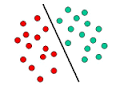
\includegraphics[scale = 0.4,trim={0.5cm 0 0.5cm 0},clip]{images/svm.png}};
	
		\draw[red!100,fill=red!10,thick,solid,rounded corners=10pt] (6,6.7) rectangle (7,9.8);
	
		\node [hidden_neuron] (neuron51) at (6.5,9.2) {} ;
		\node [hidden_neuron] (neuron52) at (6.5,8.5)  {};
		\node at (6.5,7.9) {\vdots};
		\node [hidden_neuron] (neuron53) at (6.5,7.2)  {};
		\node [cpy_neuron] (neuron01) at (6.5,8.5) {};
	
		\draw [->] (I) -- (neuron01);
		\draw  (2.7,6) -- (2.7,7);
		\draw  (2.7,7) -- (4.2,7);
		\draw [->]  (4.2,7) -- (4.2,7.8);
		\draw[draw=gray,fill=gray,opacity=0.5,thick,solid,rounded corners] (3.6,10) rectangle (7.2,6.5);
	}
	
	
	\onslide<1->{
	
		
		\node [text width = 30mm] (F) at (5.3,5.6) {Bounding Box Regression};
	
		\node[inner sep=0pt] (A) at (5.2,4.2)
		{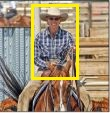
\includegraphics[scale = 0.6]{images/cowboy_cr.jpg}};
	
		\draw  (1.6,5.5) -- (1.6,4);
		\draw [->] (1.6,4) -- (4.2,4);
		\draw[draw=gray,fill=gray,opacity=0.5,thick,solid,rounded corners] (3.6,3.1) rectangle (7.2,6.2);   
	}

\end{tikzpicture}
	\end{center}
	\begin{columns}
		\column{0.5\textwidth}
		\begin{overlayarea}{\textwidth}{\textheight}
			\begin{center}
				\begin{tikzpicture}

	\onslide<2->{
		\draw[draw=blue!50,fill=cyan!10,thick,solid,rounded corners] (3.2,4.6) rectangle (0.8,7.3);

		\node[inner sep=0pt] (A) at (2,6)
		{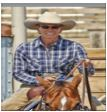
\includegraphics[scale=0.7]{images/CNN_cowboy_scale.JPG}};
	}
	
	\onslide<3->{
		\draw[draw=blue!50,fill=cyan!10,thick,solid,rounded corners] (8.5,4.6) rectangle (3.8,7.3);
		\draw[black, thick, ->]  (3,5.8) --  (4,5.8);
		\node[inner sep=0pt] (C) at (6.2,6) {\begin{tikzpicture}[thick,scale=0.8, every node/.style={scale=0.8}]     
			\pgfsetxvec{\pgfpoint{1cm}{0cm}}
			\pgfsetyvec{\pgfpoint{0cm}{1cm}}
			\pgfsetzvec{\pgfpoint{-0.707cm}{.707cm}}     
       
			\onslide<1->{
				\cuboid{(5.9,-2,0.2)}{pink!50}{0.8}{0.8}{0}
				\cuboid{(5.9,-2,0.0)}{pink!50}{0.8}{0.8}{0}
				\cuboid{(5.9,-2,-0.2)}{pink!50}{0.8}{0.8}{0}
				\cuboid{(5.9,-2,-0.4)}{pink!50}{0.8}{0.8}{0}
				\cuboid{(5.9,-2,-0.6)}{pink!50}{0.8}{0.8}{0}
				\cuboid{(5.9,-2,-0.8)}{pink!50}{0.8}{0.8}{0}
				\cuboid{(5.9,-2,-1)}{pink!50}{0.8}{0.8}{0}
				\cuboid{(5.9,-2,-1.2)}{pink!50}{0.8}{0.8}{0}
				\cuboidlabelmine{(5.9,-2,-1.2)}{pink!50}{0.8}{0.8}{0}{10}{10}{}
			}
			\onslide<1->{
             
				\cuboid{(7.9,-2.7,0.8)}{blue!50}{0.5}{0.5}{0}
				\cuboid{(7.9,-2.7,0.6)}{blue!50}{0.5}{0.5}{0}
				\cuboid{(7.9,-2.7,0.4)}{blue!50}{0.5}{0.5}{0}
				\cuboid{(7.9,-2.7,0.2)}{blue!50}{0.5}{0.5}{0}
				\cuboid{(7.9,-2.7,-0.0)}{blue!50}{0.5}{0.5}{0}
				\cuboid{(7.9,-2.7,-0.2)}{blue!50}{0.5}{0.5}{0}
				\cuboid{(7.9,-2.7,-0.4)}{blue!50}{0.5}{0.5}{0}
				\cuboid{(7.9,-2.7,-0.6)}{blue!50}{0.5}{0.5}{0}
				\cuboidlabelmine{(7.9,-2.7,-0.6)}{blue!50}{0.5}{0.5}{0}{5}{5}{}
				\kernel{(6.1,-3,-0.4)}{gray}{0.2}{0.2}{0}{(7.8,-3.2,-0.4)}
			}
			\onslide<1->{
             
				\cuboid{(9.8,-3.5,1.8)}{magenta!50}{0.5}{0}{1.4}
				%   \node at (9.3,-2.85,2.2) {\tiny{FC 1}};
				\draw[black] (7.9,-2.7,0.8) -- (9.55,-3.5,1.78);
				\draw[black] (7.9,-2.7,-0.6) -- (8.8,-3,-0.3);
			}
			\onslide<1->{
				\cuboid{(10.8,-3.5,1.7)}{magenta!50}{0.5}{0}{1.15}
             
				\draw[black] (9.8,-3.5,1.8) -- (10.5,-3.5,1.7);
				\draw[black] (9.8,-3.5,0.4) -- (10.3,-3.5,0.55);
			}
			
			\end{tikzpicture}}; 
		\node at (7.65,6.6) {fc7};
	}

\end{tikzpicture}

			\end{center}
		\end{overlayarea}
		\column{0.5\textwidth}
		\begin{overlayarea}{\textwidth}{\textheight}
			\begin{center}
				\vspace{-0.3cm}
				\begin{itemize}
					\justifying
					\item<1-> For feature extraction any CNN trained for Image Classification can be used (AlexNet/ VGGNet etc.)
					\item<2-> Outputs from fc7 layer are taken as features
					\item<3-> CNN is fine tuned using ground truth (cropped) object images
				\end{itemize}
			\end{center}
		\end{overlayarea}
	\end{columns}

\end{frame}

%%%%%%%%%%%%%%%%%%%%%%%%%%%%%%%%%%%%%%%%%%%%%%%%%%%%%%%%%%%%%%%%%%%%%%%%%%%%%%

\begin{frame}
	\begin{center}
		\begin{tikzpicture}[thick,scale=0.6, every node/.style={scale=0.6}]

	\onslide<1->{ % node[below=2]

		\node [text width = 20mm] (F) at (-6.5,7.5) {Input};
		\node[inner sep=0pt] (A) at (-7,6)
		{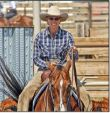
\includegraphics[scale=0.8]{images/cowboy.JPG}};
		\draw[draw=gray,fill=gray,opacity=0.5,thick,solid,rounded corners] (-8.5,4.5) rectangle (-5.5,8);   

	}

	\onslide<1->{

		\node [text width = 30mm] (F) at (-2.7,7.5) {Region Proposals};
		\node[inner sep=0pt] (B) at (-3.5,6)
		{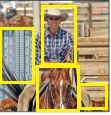
\includegraphics[scale=0.8]{images/c2.jpg}};
		\draw[black, thick, ->] (A) -- (B);     

		\node[inner sep=0pt] (C) at (-1.5,6)
		{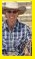
\includegraphics[]{images/c2_crop.jpg}};
		\draw[black,dashed, thick, ->] (-3,6.8) -- (C);     
		\draw[gray,dashed,->] (-3,6) -- (C);      
		\draw[gray,dashed,->] (-3,5) -- (C);     
		\draw[draw=gray,fill=gray,opacity=0.5,thick,solid,rounded corners] (-5,4.5) rectangle (-0.8,8);     
	}
	
	\onslide<1->{
		
		\node [text width = 30mm] (F) at (1.5,7.5) {Feature Extraction};
		\node[inner sep=0pt] (D) at (1.4,6)
		{\begin{tikzpicture}[thick,scale=0.6, every node/.style={scale=0.6}]     
			\pgfsetxvec{\pgfpoint{1cm}{0cm}}
			\pgfsetyvec{\pgfpoint{0cm}{1cm}}
			\pgfsetzvec{\pgfpoint{-0.707cm}{.707cm}}     

			\onslide<1->{
				\cuboid{(5.9,-2,0.2)}{pink!50}{0.8}{0.8}{0}
				\cuboid{(5.9,-2,0.0)}{pink!50}{0.8}{0.8}{0}
				\cuboid{(5.9,-2,-0.2)}{pink!50}{0.8}{0.8}{0}
				\cuboid{(5.9,-2,-0.4)}{pink!50}{0.8}{0.8}{0}
				\cuboid{(5.9,-2,-0.6)}{pink!50}{0.8}{0.8}{0}
				\cuboid{(5.9,-2,-0.8)}{pink!50}{0.8}{0.8}{0}
				\cuboid{(5.9,-2,-1)}{pink!50}{0.8}{0.8}{0}
				\cuboid{(5.9,-2,-1.2)}{pink!50}{0.8}{0.8}{0}
				\cuboidlabelmine{(5.9,-2,-1.2)}{pink!50}{0.8}{0.8}{0}{10}{10}{}
			}
			\onslide<1->{
      
				\cuboid{(7.9,-2.7,0.8)}{blue!50}{0.5}{0.5}{0}
				\cuboid{(7.9,-2.7,0.6)}{blue!50}{0.5}{0.5}{0}
				\cuboid{(7.9,-2.7,0.4)}{blue!50}{0.5}{0.5}{0}
				\cuboid{(7.9,-2.7,0.2)}{blue!50}{0.5}{0.5}{0}
				\cuboid{(7.9,-2.7,-0.0)}{blue!50}{0.5}{0.5}{0}
				\cuboid{(7.9,-2.7,-0.2)}{blue!50}{0.5}{0.5}{0}
				\cuboid{(7.9,-2.7,-0.4)}{blue!50}{0.5}{0.5}{0}
				\cuboid{(7.9,-2.7,-0.6)}{blue!50}{0.5}{0.5}{0}
				\cuboidlabelmine{(7.9,-2.7,-0.6)}{blue!50}{0.5}{0.5}{0}{5}{5}{}
				\kernel{(6.1,-3,-0.4)}{gray}{0.2}{0.2}{0}{(7.8,-3.2,-0.4)}
			}
			\onslide<1->{
      
				\cuboid{(9.8,-3.5,1.8)}{magenta!50}{0.5}{0}{1.4}
				%   \node at (9.3,-2.85,2.2) {\tiny{FC 1}};
				\draw[black] (7.9,-2.7,0.8) -- (9.55,-3.5,1.78);
				\draw[black] (7.9,-2.7,-0.6) -- (8.8,-3,-0.3);
			}
			\onslide<1->{
				\cuboid{(10.8,-3.5,1.7)}{magenta!50}{0.5}{0}{1.15}
      
				\draw[black] (9.8,-3.5,1.8) -- (10.5,-3.5,1.7);
				\draw[black] (9.8,-3.5,0.4) -- (10.3,-3.5,0.55);
			}
		\end{tikzpicture}};
		\draw[black, thick, ->] (C) -- (D);          
		\draw[draw=gray,fill=gray,opacity=0.5,thick,solid,rounded corners] (-0.4,4.5) rectangle (3.2,8);
	}
	
	\onslide<1->{
	
		\tikzstyle{input_neuron}=[circle,draw=red!50,fill=red!10,thick,minimum size=6mm]
		\tikzstyle{hidden_neuron}=[circle,draw=blue!50,fill=cyan!10,thick,minimum size=6mm]
		\tikzstyle{output_neuron}=[circle,draw=green!50,fill=green!10,thick,minimum size=6mm]
		\tikzstyle{cpy_neuron}=[circle,draw=red!50,fill=red!50,thick,minimum size=6mm]
		\tikzstyle{input}=[circle,draw=black!50,fill=black!20,thick,minimum size=6mm]
	
		\draw[draw=green!50,fill=yellow,thick,solid,rounded corners] (3.6,10) rectangle (7.2,6.5);
		\node [text width = 30mm] (F) at (5.3,9.5) {Classifier};
		%    \draw (4.5,6.5) rectangle (6.5,8);
		%\node [text width = 25mm] (E) at (4.5,8.2) {Linear Classifier};
		\draw  (3.8,7.85) -- (3.8,9.1);
		\draw  (3.8,7.8) -- (5.2,7.8);
		\node[inner sep=0pt] (I) at (4.5,8.5)
		{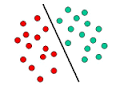
\includegraphics[scale = 0.4,trim={0.5cm 0 0.5cm 0},clip]{images/svm.png}};
	
		\draw[red!100,fill=red!10,thick,solid,rounded corners=10pt] (6,6.7) rectangle (7,9.8);
	
		\node [hidden_neuron] (neuron51) at (6.5,9.2) {} ;
		\node [hidden_neuron] (neuron52) at (6.5,8.5)  {};
		\node at (6.5,7.9) {\vdots};
		\node [hidden_neuron] (neuron53) at (6.5,7.2)  {};
		\node [cpy_neuron] (neuron01) at (6.5,8.5) {};
	
		\draw [->] (I) -- (neuron01);
		\draw  (2.7,6) -- (2.7,7);
		\draw  (2.7,7) -- (4.2,7);
		\draw [->]  (4.2,7) -- (4.2,7.8);
	}
	
	
	\onslide<1->{
	
		\draw[draw=gray,fill=gray,opacity=0.5,thick,solid,rounded corners] (3.6,3.1) rectangle (7.2,6.2);
		\node [text width = 30mm] (F) at (5.3,5.6) {Bounding Box Regression};
	
		\node[inner sep=0pt] (A) at (5.2,4.2)
		{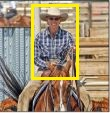
\includegraphics[scale = 0.6]{images/cowboy_cr.jpg}};
	
		\draw  (1.6,5.5) -- (1.6,4);
		\draw [->] (1.6,4) -- (4.2,4);
	}

\end{tikzpicture}

	\end{center}
	\begin{overlayarea}{\textwidth}{\textheight}
		\begin{center}
			\begin{tikzpicture}
	\onslide<2->{
		\node[inner sep=0pt] (D) at (2,2)
		{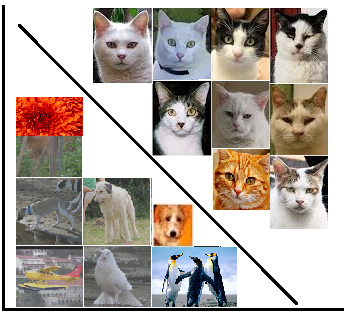
\includegraphics[scale=0.35]{images/cats.png}}; 
	}
	
	\onslide<3->{
		\node[inner sep=0pt] (E) at (6,2)
		{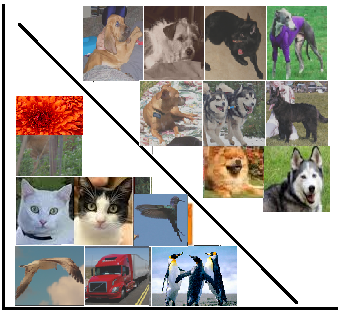
\includegraphics[scale=0.35]{images/dogs_fin.png}}; 
	}
	\onslide<4->{ \node at (8.5,2) {\dots};}
	\onslide<5->{
		\node[inner sep=0pt] (E) at (11,2)
		{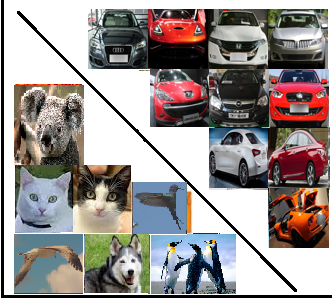
\includegraphics[scale=0.35]{images/cars.png}}; 
	}
\end{tikzpicture}	
		\end{center}
		\vspace{-0.5cm}
		\begin{itemize}
			\item<2->Linear models (SVMs) are used for classification \onslide<3->{(1 model per class)}
		\end{itemize}
		
	\end{overlayarea}
\end{frame}

%%%%%%%%%%%%%%%%%%%%%%%%%%%%%%%%%%%%%%%%%%%%%%%%%%%%%%%%%%%%%%%%%%%%%%%%%%%%%%

\begin{frame}
	\begin{center}
		\begin{tikzpicture}[thick,scale=0.5, every node/.style={scale=0.5}]

	\onslide<1->{ % node[below=2]

		\node [text width = 20mm] (F) at (-6.5,7.5) {Input};
		\node[inner sep=0pt] (A) at (-7,6)
		{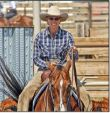
\includegraphics[scale=0.8]{images/cowboy.JPG}};
		\draw[draw=gray,fill=gray,opacity=0.5,thick,solid,rounded corners] (-8.5,4.5) rectangle (-5.5,8);   

	}

	\onslide<1->{

		\node [text width = 30mm] (F) at (-2.7,7.5) {Region Proposals};
		\node[inner sep=0pt] (B) at (-3.5,6)
		{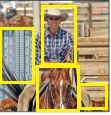
\includegraphics[scale=0.8]{images/c2.jpg}};
		\draw[black, thick, ->] (A) -- (B);     

		\node[inner sep=0pt] (C) at (-1.5,6)
		{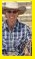
\includegraphics[]{images/c2_crop.jpg}};
		\draw[black,dashed, thick, ->] (-3,6.8) -- (C);     
		\draw[gray,dashed,->] (-3,6) -- (C);      
		\draw[gray,dashed,->] (-3,5) -- (C);     
		\draw[draw=gray,fill=gray,opacity=0.5,thick,solid,rounded corners] (-5,4.5) rectangle (-0.8,8);     
	}

	\onslide<1->{

		\node [text width = 30mm] (F) at (1.5,7.5) {Feature Extraction};
		\node[inner sep=0pt] (D) at (1.4,6)
		{\begin{tikzpicture}[thick,scale=0.6, every node/.style={scale=0.6}]     
			\pgfsetxvec{\pgfpoint{1cm}{0cm}}
			\pgfsetyvec{\pgfpoint{0cm}{1cm}}
			\pgfsetzvec{\pgfpoint{-0.707cm}{.707cm}}     
   
			\onslide<1->{
				\cuboid{(5.9,-2,0.2)}{pink!50}{0.8}{0.8}{0}
				\cuboid{(5.9,-2,0.0)}{pink!50}{0.8}{0.8}{0}
				\cuboid{(5.9,-2,-0.2)}{pink!50}{0.8}{0.8}{0}
				\cuboid{(5.9,-2,-0.4)}{pink!50}{0.8}{0.8}{0}
				\cuboid{(5.9,-2,-0.6)}{pink!50}{0.8}{0.8}{0}
				\cuboid{(5.9,-2,-0.8)}{pink!50}{0.8}{0.8}{0}
				\cuboid{(5.9,-2,-1)}{pink!50}{0.8}{0.8}{0}
				\cuboid{(5.9,-2,-1.2)}{pink!50}{0.8}{0.8}{0}
				\cuboidlabelmine{(5.9,-2,-1.2)}{pink!50}{0.8}{0.8}{0}{10}{10}{}
			}
			\onslide<1->{
         
				\cuboid{(7.9,-2.7,0.8)}{blue!50}{0.5}{0.5}{0}
				\cuboid{(7.9,-2.7,0.6)}{blue!50}{0.5}{0.5}{0}
				\cuboid{(7.9,-2.7,0.4)}{blue!50}{0.5}{0.5}{0}
				\cuboid{(7.9,-2.7,0.2)}{blue!50}{0.5}{0.5}{0}
				\cuboid{(7.9,-2.7,-0.0)}{blue!50}{0.5}{0.5}{0}
				\cuboid{(7.9,-2.7,-0.2)}{blue!50}{0.5}{0.5}{0}
				\cuboid{(7.9,-2.7,-0.4)}{blue!50}{0.5}{0.5}{0}
				\cuboid{(7.9,-2.7,-0.6)}{blue!50}{0.5}{0.5}{0}
				\cuboidlabelmine{(7.9,-2.7,-0.6)}{blue!50}{0.5}{0.5}{0}{5}{5}{}
				\kernel{(6.1,-3,-0.4)}{gray}{0.2}{0.2}{0}{(7.8,-3.2,-0.4)}
			}
			\onslide<1->{
         
				\cuboid{(9.8,-3.5,1.8)}{magenta!50}{0.5}{0}{1.4}
				%   \node at (9.3,-2.85,2.2) {\tiny{FC 1}};
				\draw[black] (7.9,-2.7,0.8) -- (9.55,-3.5,1.78);
				\draw[black] (7.9,-2.7,-0.6) -- (8.8,-3,-0.3);
			}
			\onslide<1->{
				\cuboid{(10.8,-3.5,1.7)}{magenta!50}{0.5}{0}{1.15}
         
				\draw[black] (9.8,-3.5,1.8) -- (10.5,-3.5,1.7);
				\draw[black] (9.8,-3.5,0.4) -- (10.3,-3.5,0.55);
			}
		\end{tikzpicture}};
		\draw[black, thick, ->] (C) -- (D);          
		\draw[draw=gray,fill=gray,opacity=0.5,thick,solid,rounded corners] (-0.4,4.5) rectangle (3.2,8);
	}
	
	\onslide<1->{
	
		\tikzstyle{input_neuron}=[circle,draw=red!50,fill=red!10,thick,minimum size=6mm]
		\tikzstyle{hidden_neuron}=[circle,draw=blue!50,fill=cyan!10,thick,minimum size=6mm]
		\tikzstyle{output_neuron}=[circle,draw=green!50,fill=green!10,thick,minimum size=6mm]
		\tikzstyle{cpy_neuron}=[circle,draw=red!50,fill=red!50,thick,minimum size=6mm]
		\tikzstyle{input}=[circle,draw=black!50,fill=black!20,thick,minimum size=6mm]
	
		
		\node [text width = 30mm] (F) at (5.3,9.5) {Classifier};
		%    \draw (4.5,6.5) rectangle (6.5,8);
		%\node [text width = 25mm] (E) at (4.5,8.2) {Linear Classifier};
		\draw  (3.8,7.85) -- (3.8,9.1);
		\draw  (3.8,7.8) -- (5.2,7.8);
		\node[inner sep=0pt] (I) at (4.5,8.5)
		{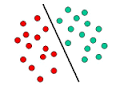
\includegraphics[scale = 0.4,trim={0.5cm 0 0.5cm 0},clip]{images/svm.png}};
	
		\draw[red!100,fill=red!10,thick,solid,rounded corners=10pt] (6,6.7) rectangle (7,9.8);
	
		\node [hidden_neuron] (neuron51) at (6.5,9.2) {} ;
		\node [hidden_neuron] (neuron52) at (6.5,8.5)  {};
		\node at (6.5,7.9) {\vdots};
		\node [hidden_neuron] (neuron53) at (6.5,7.2)  {};
		\node [cpy_neuron] (neuron01) at (6.5,8.5) {};
	
		\draw [->] (I) -- (neuron01);
		\draw  (2.7,6) -- (2.7,7);
		\draw  (2.7,7) -- (4.2,7);
		\draw [->]  (4.2,7) -- (4.2,7.8);
		\draw[draw=gray,fill=gray,opacity=0.5,thick,solid,rounded corners] (3.6,10) rectangle (7.2,6.5);
	}
	
	
	
	\onslide<1->{
	
		\draw[draw=green!50,fill=yellow,thick,solid,rounded corners] (3.6,3.1) rectangle (7.2,6.2);
		\node [text width = 30mm] (F) at (5.3,5.6) {Bounding Box Regression};
	
		\node[inner sep=0pt] (A) at (5.2,4.2)
		{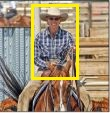
\includegraphics[scale = 0.6]{images/cowboy_cr.jpg}};
	
		\draw  (1.6,5.5) -- (1.6,4);
		\draw [->] (1.6,4) -- (4.2,4);
	}

\end{tikzpicture}

	\end{center}
	
	\begin{columns}
		\column{0.3\textwidth}
		\begin{overlayarea}{\textwidth}{\textheight}
			\vspace{0.5cm}
			\begin{center}
				\begin{tikzpicture}[scale=0.7, transform shape]
	\onslide<2->{

		\draw[draw=green!50,fill=green!10,thick,solid,rounded corners] (3.4,0.6) rectangle (0.6,3.4);

		\node[inner sep=0pt] (D) at (2,2)
		{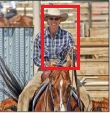
\includegraphics[scale=0.8]{images/cowboy_pred.jpg}};
		\draw [draw=yellow,fill=yellow] (2.15,2.4) circle (0.06);    
		\node[yellow] at (2.15,2.2) {($x$,$y$)};     
		\node[yellow] at (2,1.5) {$w$};
		\node[yellow] at (1.5,2.4) {$h$};
		\node at (2,0) {Proposed Box};
	}
	
	\onslide<3->{
		\draw[draw=green!50,fill=green!10,thick,solid,rounded corners] (7.4,0.6) rectangle (4.6,3.4);

		\node[inner sep=0pt] (E) at (6,2)
		{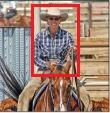
\includegraphics[scale=0.8]{images/cowboy_true.jpg}}; 
		\node[yellow] at (6,1.4) {$w^*$};     
		\node[yellow] at (5.4,2.4) {$h^*$};
		\draw [draw=yellow,fill=yellow] (6.1,2.4) circle (0.06);    
		
		\node[yellow] at (6.1,2.2) {($x^*$,$y^*$)};     
		\node at (6,0) {True Box};
	}
	
	\onslide<6->{\node at (4.1,-0.6) {z : features from pool5 layer of the network};
	}
\end{tikzpicture}

			\end{center}
		\end{overlayarea}
		
		\column{0.7\textwidth}
		\begin{overlayarea}{\textwidth}{\textheight}
			\vspace{-0.3cm}
			
			\only<3-5>{ \color{white}{\[\min \sum_{i=1}^{N} \frac{x^* - x}{w} - w_1^Tz  \]}
				\vspace{-0.5cm} 
				\begin{itemize}
					\justifying
					\item<3-> The proposed regions may not be perfect  
					\item<4-> We want to learn four regression models which will learn to predict $x^*$, $y^*$, $w^*,\ h^*$
					\item<5-> We will see their respective objective functions
				\end{itemize}
			}
			\only<6-10>{ \[\min \sum_{i=1}^{N} \Big(\frac{x^* - x}{w} - w_1^Tz\Big)^{2} \]
				\vspace{-0.5cm} 
				\begin{itemize}
					\justifying
					\item<7->  $\frac{x^* - x}{w}$ is the normalized difference between proposed $x$ and true $x^*$
					\item<8-> If we can predict this difference we can compute $x^*$
					\item<9-> The model predicts $w_1^Tz$ as this difference
					\item<10-> The above objective function minimize the difference between the predicted and the actual value
				\end{itemize}
			}
			
			\only<11>{ \[\min \sum_{i=1}^{N} \Big( \frac{y^* - y}{h} - w_2^Tz \Big)^{2}\]
				\vspace{-0.5cm} 
				\begin{itemize}
					\item<11>  Similarly for $y$
				\end{itemize}
			}
			
			\only<12>{ \[\min \sum_{i=1}^{N} \Big( \ln \Big( \frac{w^*}{w} \Big) - w_3^Tz \Big)^{2} \]
				\vspace{-0.5cm} 
				\begin{itemize}
					\item<12>  Similarly for $w$
				\end{itemize}
			}
			
			
			
			\only<13>{ \[\min \sum_{i=1}^{N} \Big( \ln \Big( \frac{h^*}{h} \Big) - w_4^Tz \Big)^{2} \]
				\vspace{-0.5cm} 
				\begin{itemize}
					\item<13>  Similarly for $h$
 
				\end{itemize}
			}

		\end{overlayarea}
	\end{columns}
\end{frame}

%%%%%%%%%%%%%%%%%%%%%%%%%%%%%%%%%%%%%%%%%%%%%%%%%%%%%%%%%%%%%%%%%%%%%%%%%%%%%%

\begin{frame}
	\begin{center}
		\begin{tikzpicture}[thick,scale=0.6, every node/.style={scale=0.6}]
     
	\onslide<1->{ % node[below=2]
       
		\draw[draw=red!50,fill=red!10,thick,solid,rounded corners] (-8.5,4.5) rectangle (-5.5,8); 
		\node [text width = 20mm] (F) at (-6.5,7.5) {Input};
		\node[inner sep=0pt] (A) at (-7,6)
		{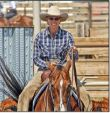
\includegraphics[scale=0.8]{images/cowboy.JPG}};
       
	}
 
 
	\onslide<1->{ 
		\draw[draw=yellow!50,fill=cyan!10,thick,solid,rounded corners] (-5,4.5) rectangle (-2,8); 
		\node [text width = 30mm] (F) at (-3.3,7.5) {Region Proposals};
		\node[inner sep=0pt] (B) at (-3.5,6)
		{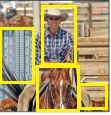
\includegraphics[scale=0.8]{images/c2.jpg}};
		\draw[black, thick, ->] (A) -- (B);     
	}
 
	\onslide<1->{
		\draw[draw=blue!50,fill=cyan!10,thick,solid,rounded corners] (-5,4.5) rectangle (-0.8,8); 
		\node [text width = 30mm] (F) at (-2.7,7.5) {Region Proposals};
		\node[inner sep=0pt] (B) at (-3.5,6)
		{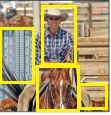
\includegraphics[scale=0.8]{images/c2.jpg}};
		\draw[black, thick, ->] (A) -- (B);     
       
		\node[inner sep=0pt] (C) at (-1.5,6)
		{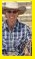
\includegraphics[]{images/c2_crop.jpg}};
		\draw[black,dashed, thick, ->] (-3,6.8) -- (C);     
		\draw[gray,dashed,->] (-3,6) -- (C);      
		\draw[gray,dashed,->] (-3,5) -- (C);     
	}
 
	\onslide<1->{
       
		\draw[draw=blue!50,fill=cyan!10,thick,solid,rounded corners] (-0.4,4.5) rectangle (3.2,8);
		\node [text width = 30mm] (F) at (1.5,7.5) {Feature Extraction};
		\node[inner sep=0pt] (D) at (1.4,6)
		{\begin{tikzpicture}[thick,scale=0.6, every node/.style={scale=0.6}]     
			\pgfsetxvec{\pgfpoint{1cm}{0cm}}
			\pgfsetyvec{\pgfpoint{0cm}{1cm}}
			\pgfsetzvec{\pgfpoint{-0.707cm}{.707cm}}     
             
			\onslide<1->{
				\cuboid{(5.9,-2,0.2)}{pink!50}{0.8}{0.8}{0}
				\cuboid{(5.9,-2,0.0)}{pink!50}{0.8}{0.8}{0}
				\cuboid{(5.9,-2,-0.2)}{pink!50}{0.8}{0.8}{0}
				\cuboid{(5.9,-2,-0.4)}{pink!50}{0.8}{0.8}{0}
				\cuboid{(5.9,-2,-0.6)}{pink!50}{0.8}{0.8}{0}
				\cuboid{(5.9,-2,-0.8)}{pink!50}{0.8}{0.8}{0}
				\cuboid{(5.9,-2,-1)}{pink!50}{0.8}{0.8}{0}
				\cuboid{(5.9,-2,-1.2)}{pink!50}{0.8}{0.8}{0}
				\cuboidlabelmine{(5.9,-2,-1.2)}{pink!50}{0.8}{0.8}{0}{10}{10}{}
			}
			\onslide<1->{
                   
				\cuboid{(7.9,-2.7,0.8)}{blue!50}{0.5}{0.5}{0}
				\cuboid{(7.9,-2.7,0.6)}{blue!50}{0.5}{0.5}{0}
				\cuboid{(7.9,-2.7,0.4)}{blue!50}{0.5}{0.5}{0}
				\cuboid{(7.9,-2.7,0.2)}{blue!50}{0.5}{0.5}{0}
				\cuboid{(7.9,-2.7,-0.0)}{blue!50}{0.5}{0.5}{0}
				\cuboid{(7.9,-2.7,-0.2)}{blue!50}{0.5}{0.5}{0}
				\cuboid{(7.9,-2.7,-0.4)}{blue!50}{0.5}{0.5}{0}
				\cuboid{(7.9,-2.7,-0.6)}{blue!50}{0.5}{0.5}{0}
				\cuboidlabelmine{(7.9,-2.7,-0.6)}{blue!50}{0.5}{0.5}{0}{5}{5}{}
				\kernel{(6.1,-3,-0.4)}{gray}{0.2}{0.2}{0}{(7.8,-3.2,-0.4)}
			}
			\onslide<1->{
                   
				\cuboid{(9.8,-3.5,1.8)}{magenta!50}{0.5}{0}{1.4}
				%   \node at (9.3,-2.85,2.2) {\tiny{FC 1}};
				\draw[black] (7.9,-2.7,0.8) -- (9.55,-3.5,1.78);
				\draw[black] (7.9,-2.7,-0.6) -- (8.8,-3,-0.3);
			}
			\onslide<1->{
				\cuboid{(10.8,-3.5,1.7)}{magenta!50}{0.5}{0}{1.15}
                   
				\draw[black] (9.8,-3.5,1.8) -- (10.5,-3.5,1.7);
				\draw[black] (9.8,-3.5,0.4) -- (10.3,-3.5,0.55);
			}
		\end{tikzpicture}};
		\draw[black, thick, ->] (C) -- (D);          
	}
	\onslide<2-> {
		\node [text width = 30mm] (F) at (1.7,8.5) {$W_{CONV}$};
		\node [text width = 30mm] (K) at (9,8.6) {$W_{classifier}$};
		\node [text width = 30mm] (L) at (9,4.6) {$W_{regression}$};
	}
         
	\onslide<1->{
          
		\tikzstyle{input_neuron}=[circle,draw=red!50,fill=red!10,thick,minimum size=6mm]
		\tikzstyle{hidden_neuron}=[circle,draw=blue!50,fill=cyan!10,thick,minimum size=6mm]
		\tikzstyle{output_neuron}=[circle,draw=green!50,fill=green!10,thick,minimum size=6mm]
		\tikzstyle{cpy_neuron}=[circle,draw=red!50,fill=red!50,thick,minimum size=6mm]
		\tikzstyle{input}=[circle,draw=black!50,fill=black!20,thick,minimum size=6mm]
          
		\draw[draw=green!50,fill=yellow!40,thick,solid,rounded corners] (3.6,10) rectangle (7.2,6.5);
		\node [text width = 30mm] (F) at (5.3,9.5) {Classifier};
		%    \draw (4.5,6.5) rectangle (6.5,8);
		%\node [text width = 25mm] (E) at (4.5,8.2) {Linear Classifier};
		\draw  (3.8,7.85) -- (3.8,9.1);
		\draw  (3.8,7.8) -- (5.2,7.8);
		\node[inner sep=0pt] (I) at (4.5,8.5)
		{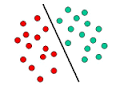
\includegraphics[scale = 0.4,trim={0.5cm 0 0.5cm 0},clip]{images/svm.png}};
          
		\draw[red!100,fill=red!10,thick,solid,rounded corners=10pt] (6,6.7) rectangle (7,9.8);
          
		\node [hidden_neuron] (neuron51) at (6.5,9.2) {} ;
		\node [hidden_neuron] (neuron52) at (6.5,8.5)  {};
		\node at (6.5,7.9) {\vdots};
		\node [hidden_neuron] (neuron53) at (6.5,7.2)  {};
		\node [cpy_neuron] (neuron01) at (6.5,8.5) {};
          
		\draw [->] (I) -- (neuron01);
		\draw  (2.7,6) -- (2.7,7);
		\draw  (2.7,7) -- (4.2,7);
		\draw [->]  (4.2,7) -- (4.2,7.8);
	}
    
    
	\onslide<1->{
          
		\draw[draw=green!50,fill=green!10,thick,solid,rounded corners] (3.6,3.1) rectangle (7.2,6.2);
		\node [text width = 30mm] (F) at (5.3,5.6) {Bounding Box Regression};
          
		\node[inner sep=0pt] (A) at (5.2,4.2)
		{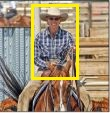
\includegraphics[scale = 0.6]{images/cowboy_cr.jpg}};
          
		\draw  (1.6,5.5) -- (1.6,4);
		\draw [->] (1.6,4) -- (4.2,4);
	}
    
\end{tikzpicture}

	\end{center}

	\begin{overlayarea}{\textwidth}{\textheight}
		
		\only<1->{
			\begin{itemize}
				\justifying
				\item<1-> What are the parameters of this model?
				\item<3-> $W_{CONV}$ is taken as it is from a CNN trained for Image classification (say on ImageNet)
				\item<4-> $W_{CONV}$ is then fine tuned using ground truth (cropped) object images
				\item<5-> $W_{classifier}$ is learned using ground truth (cropped) object images
				\item<6> $W_{regression}$ is learned using ground truth bounding boxes
			\end{itemize}
		}
	\end{overlayarea}
\end{frame}

%%%%%%%%%%%%%%%%%%%%%%%%%%%%%%%%%%%%%%%%%%%%%%%%%%%%%%%%%%%%%%%%%%%%%%%%%%%%%%

\begin{frame}
	\begin{center}
		\begin{tikzpicture}[thick,scale=0.6, every node/.style={scale=0.6}]
 
	\onslide<1->{ % node[below=2]
       
		\draw[draw=red!50,fill=red!10,thick,solid,rounded corners] (-8.5,4.5) rectangle (-5.5,8); 
		\node [text width = 20mm] (F) at (-6.5,7.5) {Input};
		\node[inner sep=0pt] (A) at (-7,6)
		{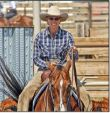
\includegraphics[scale=0.8]{images/cowboy.JPG}};
       
	}
 
 
	\onslide<1->{ 
		\draw[draw=yellow!50,fill=cyan!10,thick,solid,rounded corners] (-5,4.5) rectangle (-2,8); 
		\node [text width = 30mm] (F) at (-3.3,7.5) {Region Proposals};
		\node[inner sep=0pt] (B) at (-3.5,6)
		{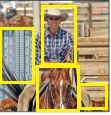
\includegraphics[scale=0.8]{images/c2.jpg}};
		\draw[black, thick, ->] (A) -- (B);     
	}
 
	\onslide<1->{
		\draw[draw=blue!50,fill=cyan!10,thick,solid,rounded corners] (-5,4.5) rectangle (-0.8,8); 
		\node [text width = 30mm] (F) at (-2.7,7.5) {Region Proposals};
		\node[inner sep=0pt] (B) at (-3.5,6)
		{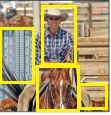
\includegraphics[scale=0.8]{images/c2.jpg}};
		\draw[black, thick, ->] (A) -- (B);     
       
		\node[inner sep=0pt] (C) at (-1.5,6)
		{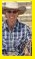
\includegraphics[]{images/c2_crop.jpg}};
		\draw[black,dashed, thick, ->] (-3,6.8) -- (C);     
		\draw[gray,dashed,->] (-3,6) -- (C);      
		\draw[gray,dashed,->] (-3,5) -- (C);     
	}
 
	\onslide<1->{
		\draw[draw=blue!50,fill=cyan!10,thick,solid,rounded corners] (-0.4,4.5) rectangle (3.2,8);
		\node [text width = 30mm] (F) at (1.5,7.5) {Feature Extraction};
		\node[inner sep=0pt] (D) at (1.4,6)
		{\begin{tikzpicture}[thick,scale=0.6, every node/.style={scale=0.6}]     
			\pgfsetxvec{\pgfpoint{1cm}{0cm}}
			\pgfsetyvec{\pgfpoint{0cm}{1cm}}
			\pgfsetzvec{\pgfpoint{-0.707cm}{.707cm}}     
             
			\onslide<1->{
				\cuboid{(5.9,-2,0.2)}{pink!50}{0.8}{0.8}{0}
				\cuboid{(5.9,-2,0.0)}{pink!50}{0.8}{0.8}{0}
				\cuboid{(5.9,-2,-0.2)}{pink!50}{0.8}{0.8}{0}
				\cuboid{(5.9,-2,-0.4)}{pink!50}{0.8}{0.8}{0}
				\cuboid{(5.9,-2,-0.6)}{pink!50}{0.8}{0.8}{0}
				\cuboid{(5.9,-2,-0.8)}{pink!50}{0.8}{0.8}{0}
				\cuboid{(5.9,-2,-1)}{pink!50}{0.8}{0.8}{0}
				\cuboid{(5.9,-2,-1.2)}{pink!50}{0.8}{0.8}{0}
				\cuboidlabelmine{(5.9,-2,-1.2)}{pink!50}{0.8}{0.8}{0}{10}{10}{}
			}
			\onslide<1->{
                   
				\cuboid{(7.9,-2.7,0.8)}{blue!50}{0.5}{0.5}{0}
				\cuboid{(7.9,-2.7,0.6)}{blue!50}{0.5}{0.5}{0}
				\cuboid{(7.9,-2.7,0.4)}{blue!50}{0.5}{0.5}{0}
				\cuboid{(7.9,-2.7,0.2)}{blue!50}{0.5}{0.5}{0}
				\cuboid{(7.9,-2.7,-0.0)}{blue!50}{0.5}{0.5}{0}
				\cuboid{(7.9,-2.7,-0.2)}{blue!50}{0.5}{0.5}{0}
				\cuboid{(7.9,-2.7,-0.4)}{blue!50}{0.5}{0.5}{0}
				\cuboid{(7.9,-2.7,-0.6)}{blue!50}{0.5}{0.5}{0}
				\cuboidlabelmine{(7.9,-2.7,-0.6)}{blue!50}{0.5}{0.5}{0}{5}{5}{}
				\kernel{(6.1,-3,-0.4)}{gray}{0.2}{0.2}{0}{(7.8,-3.2,-0.4)}
			}
			\onslide<1->{
                   
				\cuboid{(9.8,-3.5,1.8)}{magenta!50}{0.5}{0}{1.4}
				%   \node at (9.3,-2.85,2.2) {\tiny{FC 1}};
				\draw[black] (7.9,-2.7,0.8) -- (9.55,-3.5,1.78);
				\draw[black] (7.9,-2.7,-0.6) -- (8.8,-3,-0.3);
			}
			\onslide<1->{
				\cuboid{(10.8,-3.5,1.7)}{magenta!50}{0.5}{0}{1.15}
                   
				\draw[black] (9.8,-3.5,1.8) -- (10.5,-3.5,1.7);
				\draw[black] (9.8,-3.5,0.4) -- (10.3,-3.5,0.55);
			}
		\end{tikzpicture}};
		\draw[black, thick, ->] (C) -- (D);          
	}
	
	\onslide<1->{
	      
		\tikzstyle{input_neuron}=[circle,draw=red!50,fill=red!10,thick,minimum size=6mm]
		\tikzstyle{hidden_neuron}=[circle,draw=blue!50,fill=cyan!10,thick,minimum size=6mm]
		\tikzstyle{output_neuron}=[circle,draw=green!50,fill=green!10,thick,minimum size=6mm]
		\tikzstyle{cpy_neuron}=[circle,draw=red!50,fill=red!50,thick,minimum size=6mm]
		\tikzstyle{input}=[circle,draw=black!50,fill=black!20,thick,minimum size=6mm]
	      
		\draw[draw=green!50,fill=yellow!40,thick,solid,rounded corners] (3.6,10) rectangle (7.2,6.5);
		\node [text width = 30mm] (F) at (5.3,9.5) {Classifier};
		%    \draw (4.5,6.5) rectangle (6.5,8);
		%\node [text width = 25mm] (E) at (4.5,8.2) {Linear Classifier};
		\draw  (3.8,7.85) -- (3.8,9.1);
		\draw  (3.8,7.8) -- (5.2,7.8);
		\node[inner sep=0pt] (I) at (4.5,8.5)
		{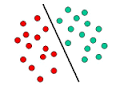
\includegraphics[scale = 0.4,trim={0.5cm 0 0.5cm 0},clip]{images/svm.png}};
	      
		\draw[red!100,fill=red!10,thick,solid,rounded corners=10pt] (6,6.7) rectangle (7,9.8);
	      
		\node [hidden_neuron] (neuron51) at (6.5,9.2) {} ;
		\node [hidden_neuron] (neuron52) at (6.5,8.5)  {};
		\node at (6.5,7.9) {\vdots};
		\node [hidden_neuron] (neuron53) at (6.5,7.2)  {};
		\node [cpy_neuron] (neuron01) at (6.5,8.5) {};
	      
		\draw [->] (I) -- (neuron01);
		\draw  (2.7,6) -- (2.7,7);
		\draw  (2.7,7) -- (4.2,7);
		\draw [->]  (4.2,7) -- (4.2,7.8);
	}
	
	
	\onslide<1->{
	      
		\draw[draw=green!50,fill=green!10,thick,solid,rounded corners] (3.6,3.1) rectangle (7.2,6.2);
		\node [text width = 30mm] (F) at (5.3,5.6) {Bounding Box Regression};
	      
		\node[inner sep=0pt] (A) at (5.2,4.2)
		{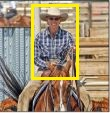
\includegraphics[scale = 0.6]{images/cowboy_cr.jpg}};
	      
		\draw  (1.6,5.5) -- (1.6,4);
		\draw [->] (1.6,4) -- (4.2,4);
	}

\end{tikzpicture}
	\end{center}

	\begin{overlayarea}{\textwidth}{\textheight}
		\begin{itemize}
			\justifying
			\item<1-> What is the computational cost for processing one image at test time?
			\item<2-> Inference Time = Proposal Time + $\#$ Proposals $\times$ Convolution Time  +  $\#$ Proposals $\times$ classification + $\#$ Proposals $\times$ regression 
		\end{itemize}

	\end{overlayarea}
\end{frame}

%%%%%%%%%%%%%%%%%%%%%%%%%%%%%%%%%%%%%%%%%%%%%%%%%%%%%%%%%%%%%%%%%%%%%%%%%%%%%%

\begin{frame}
	\vspace{1cm}
	\begin{columns}
		\column{0.6\textwidth}	
		\begin{overlayarea}{\textwidth}{\textheight}
			\begin{figure}
				\begin{overprint}
					\onslide<1>\centering\includegraphics[scale= 0.5]{images/33}\caption[Caption]{\hspace{-140pt} Source: \it{Ross Girshick}}
					\onslide<2>\centering\includegraphics[scale= 0.5]{images/34}\caption[Caption]{\hspace{-140pt} Source: \it{Ross Girshick}}
					\onslide<3>\centering\includegraphics[scale= 0.5]{images/35}\caption[Caption]{\hspace{-140pt} Source: \it{Ross Girshick}}
					\onslide<4>\centering\includegraphics[scale= 0.5]{images/36}\caption[Caption]{\hspace{-140pt} Source: \it{Ross Girshick}}
					\onslide<5>\centering\includegraphics[scale= 0.5]{images/37}\caption[Caption]{\hspace{-140pt} Source: \it{Ross Girshick}}
					\onslide<6->\centering\includegraphics[scale= 0.5]{images/38}\caption[Caption]{\hspace{-140pt} Source: \it{Ross Girshick}}
				\end{overprint}
			\end{figure}
		\end{overlayarea}
		
		\column{0.4\textwidth}
		\begin{overlayarea}{\textwidth}{\textheight}
			\begin{itemize}
				\justifying
				\item<2-> On average selective search gives 2K region proposal
				\item<4-> Each of these pass through the CNN for feature extraction 
				\item<5-> Followed by classification and regression 
			\end{itemize}
			
		\end{overlayarea}
		
	\end{columns}
\end{frame}

%%%%%%%%%%%%%%%%%%%%%%%%%%%%%%%%%%%%%%%%%%%%%%%%%%%%%%%%%%%%%%%%%%%%%%%%%%%%%%

\begin{frame}
	\begin{columns}
		\column{0.5\textwidth}
		\begin{overlayarea}{\textwidth}{\textheight}  
			\onslide<1->{\centering\includegraphics[scale= 0.2]{images/Picture1}}
		\end{overlayarea}
             
		\column{0.5\textwidth}
		\begin{overlayarea}{\textwidth}{\textheight}  
			\begin{itemize}
				\justifying
				\item No joint learning 
				\item<2-> Use ad hoc training objectives
				\begin{itemize}
			      	\justifying
			      	\item<3-> Fine tune network with softmax classifier (log loss)
			      	\item<4-> Train post-hoc linear SVMs (hinge loss)
			      	\item<5-> Train post-hoc bounding-box regressors (squared loss)
				\end{itemize}
				\item<6-> Training ($\approx$ 3 days) and testing (47s per image) is slow\footnotemark.
				\item<7-> Takes a lot of disk space
			\end{itemize}
		\end{overlayarea}
        
	\end{columns}
	\vspace{-1cm}
	\footnotetext{Source: \it{Ross Girshick} }
	\footnotetext{Using VGG-Net} 
	%\vspace{10pt}
\end{frame}

%%%%%%%%%%%%%%%%%%%%%%%%%%%%%%%%%%%%%%%%%%%%%%%%%%%%%%%%%%%%%%%%%%%%%%%%%%%%%%

\begin{frame}
	\begin{columns}
		\column{0.5\textwidth}
		\begin{overlayarea}{\textwidth}{\textheight}
			\tikzstyle{input_neuron}=[circle,draw=red!50,fill=red!10,thick,minimum size=4mm]
\tikzstyle{hidden_neuron}=[circle,draw=blue!50,fill=cyan!10,thick,minimum size=4mm]
\tikzstyle{output_neuron}=[circle,draw=green!50,fill=green!10,thick,minimum size=4mm]
\tikzstyle{cpy_neuron}=[circle,draw=red!50,fill=red!50,thick,minimum size=4mm]
\tikzstyle{input}=[circle,draw=black!50,fill=black!20,thick,minimum size=4mm]

\begin{tikzpicture}[scale=0.5, transform shape]
	
	\onslide<1->{
		\node [text width = 30mm] at (2.5,3){Region proposals};
		\node[inner sep=0pt] (A) at (2.5,1.8)
		{\includegraphics[scale = 0.9]{images/bboxes.png}};

		\node [text width = 34mm] at (6.5,3){Feature extraction};
		\node[inner sep=0pt] (A) at (6.5,2)
		{\includegraphics[scale = 0.5]{images/feature.PNG}};
		
		\node [text width = 25mm] at (11.5,3){Classifier};
		\node[inner sep=0pt] (A) at (11.0,2)
		{\includegraphics[scale = 0.5]{images/classification.PNG}};
	}
	
	\onslide<1->{
		\node [text width = 25mm] at (0,0){Pre 2012};
		\node[inner sep=0pt] (A) at (2.5,0.2)
		{\includegraphics[scale = 0.6]{images/pre_2012.png}};
		\node[inner sep=0pt] (B) at (5.9,0.2)
		{\includegraphics[scale = 0.8]{images/sift.PNG}};
		\node[inner sep=0pt] (C) at (8,0.2)
		{\includegraphics[scale = 0.6]{images/hog.PNG}};
		\node[inner sep=0pt] (D) at (11,0.4)
		{\includegraphics[scale = 0.45]{images/svm.PNG}};
	}
	

	\onslide<1->{
		\onslide<1->{\node [text width = 25mm] at (0,-1.5){RCNN};
			\node[inner sep=0pt] (A) at (2.5,-1.3)
			{\includegraphics[scale = 0.6]{images/rcnn_bbox.png}};}
		\onslide<2->{\node[inner sep=0pt] (B) at (6.8,-1.4)
			{\includegraphics[scale = 0.4]{images/cnn.PNG}};}
		\onslide<3->{\node[inner sep=0pt] (D) at (11,-1.2)
			{\includegraphics[scale = 0.45]{images/svm.PNG}};}
	}
	
\end{tikzpicture}

		\end{overlayarea}
		\column{0.5\textwidth}
		\begin{overlayarea}{\textwidth}{\textheight}
			\begin{itemize}
				\item<1-> \textbf{Region Proposals:} Selective Search
				\item<2-> \textbf{Feature Extraction:} CNNs
				\item<3-> \textbf{Classifier:} Linear 
			\end{itemize}
		\end{overlayarea}
	\end{columns}
\end{frame}

%%%%%%%%%%%%%%%%%%%%%%%%%%%%%%%%%%%%%%%%%%%%%%%%%%%%%%%%%%%%%%%%%%%%%%%%%%%%%%